\documentclass[a4paper,10pt]{article}
\usepackage{algorithm}
\usepackage{algorithmic}
\usepackage{subfig}
\usepackage{graphicx}

\begin{document}

\section{Problems}
\label{sec:problems}
\subsection{JGAP Framework}
Our first decision to program in the JGAP Framework was a really bad one. Besides the days of effort we put into setting up JGAP we also lost a lot of time
attempting to get JGAP to work. Of course JGAP did something but not at all what we wanted it to do or what we expected. \\

JGAP uses a \textit{Configuration} object in which it stores, among others the \textit{Fitness Function} object and the \textit{Population}. But also settings 
and other configurations.. This is immidiately confusing as we do not have an idea what these settings are or what how the population is build up. We also had to 
implement functions we had no need for and had to use with variables (arguments) we did not want. This was easily handled as we did not use what we did not need but when 
the results started to role in we were baffled. \\

The results were seriously dissapointing. Our population hardly evolved into something better and when it did it devolved in a matter of seconds. While the first might not
be such a big problem, the second most certainly always is as devolving is the opposite of what we want.\\

We first thought this was because our fitness function but after
we updated this function to something that we had full confidence in results were still horrible. \\

We then thought this was because of the innacuracy of our fitness function
, perhaps we missed the golden mean between time saving and accuracy? It turned out we did not. A lot of simulations and testing proved that even with more thorough 
fitness functions and more accurate fitness values de-evolving continued. \\

Our next hypothesis was that strange settings within the JGAP Framework might be the cause for the unexpected reults. After we had did some serious internet research 
and code inspectations we had to conclude that 
we had no idea what these settings were. Luckily there were thousands of options we could try but none of these options were adequately documented. For example, an 
argument suggested it would change something by it's name. But we could not know what format this argument should be, why it would suddenly print errors and more extreme, 
we could not evaluate the results as results needed hours of processing time for, most likely minimal changes. \\

An example of a weird and unwanted (by our team) function 
is the \textit{Natural Selector} object and how they are implemented by JGAP might demonstrate our troubles with this framework. At one point in time we tried to simply safe
 those chromosomes that work the best. Instead of simply setting this
we needed to create an object and add it to the \textit{Configuration} object. One would think this is not a problem but JGAP stores these \textit{Natural Selectors} 
in an ordered
chain of registered selectors. The \textit{Configuration} object can also be locked and not be unlocked once it is unlocked. And lastly, the \textit{Configuration} object
sometimes resets data to \textit{null}. Once we took care of all these problems we could start testing, but this took a lot time and results were inconclusive.\\

A short summary of our problems with JGAP.

\begin{enumerate}
    \item Learning to set up the framework and basic functioning. JAR files, buildpaths, classpaths, Eclipse. It's all very confusing.
    \item The JGAP Framework worked like a black box. Even the input is in a format what you do not want to use and somehow the output is never what you would expect. 
    \item Horrible documentation. A function needs input, but what format is this input? What does this function even do? At times, event Google could not help us 
    with this.
    \item Unecessary functions. What we want is not especially difficult and there is no need for over-complicating things. If we want to select the top X performing
    chromosomes of our population we do want to go through a chain of registred selectors or find out how or why the configuration is locked or reset. 
    \item Dismissable results. De-evolving at times without any reason.
    \item Unexpected behaviour. Some poorly chosen engineering decisions result in forced use of classes we do nothing about. For example the interface 
    \textit{IChromosome} is restricted to what interfaces are. Even though we want to store addiontal information in such a class, for example a method to create code
    from a chromosome. This is not possible but it does have a slot for the ApplicationData, which can be any object. This is object is however sometimes, seemingly
    randomly reset to \textit{null}.  
\end{enumerate}

\subsection{Leaving JGAP Framework Behind}
With more and more experience with genetic programming, it became more and more clear that what we needed did not need to be extremely complicated. In the beginning 
we were already uncertain if JGAP was the best alternative but after these experiences it became clear that it was not. In one afternoon a simple framework was written
that did exactly what we wanted. Another afternoon was used to rewrite the code into something more structured using an OOP approach. Now, with extremely well-ordered and
structured code we could start running more definitive simulations, debug and expand the potential capabilities of our robots even though we were already behind schedule
a complete week. \\

Because we were not sure if it was just JGAP or JGAPs settings that were responsible for the previously achieved
 horrible results we made sure the top performing 
chromosomes always survived by implementing algorithm \ref{alg:main}.


\begin{algorithm}
\begin{algorithmic}
\STATE Initialize Population
\WHILE{true}
    \STATE Evolve Bottom 50\%
    \STATE Evaluate Bottom 50\%
    \STATE Sort Population 
    \STATE Replace Bottom 50\% With Top 50\%
\ENDWHILE
\end{algorithmic}
\caption{Main Evolution Algorithm}
\label{alg:main}
\end{algorithm}

After the first simulations it became clear that not everything was going as well as expected. While the robots did not seem to deevolve mutated chromosomes did not seem 
to have any improvements. New fitness values were similar and sometimes low and sometimes high. This happened even though new chromosomes should be only slightly different
from the best chromosomes. Even with our newly gained debug capabilities and advantages of not using JGAP but our code we could not figure this one out. We needed
a graphical representation of the fitness values throughout the evolution process so we can easily, with one glance find out when in time what fitness value was 
achieved. This helped u a lot, also in later stages of our project. Both in debugging and performance evaluations of parameters.  \\

We plot the following three values: the biggest fitness value in red, the average fitness value of the total population in blue and the average fitness value of the 
newly mutated chromosomes in a population in green. The first results, shown in figure \ref{fig:result_1} clearly explain what is going on.\\

\begin{figure}[h!]
  \centering
  \subfloat[3.7 After 7 rounds ]{\label{fig:result_1_1}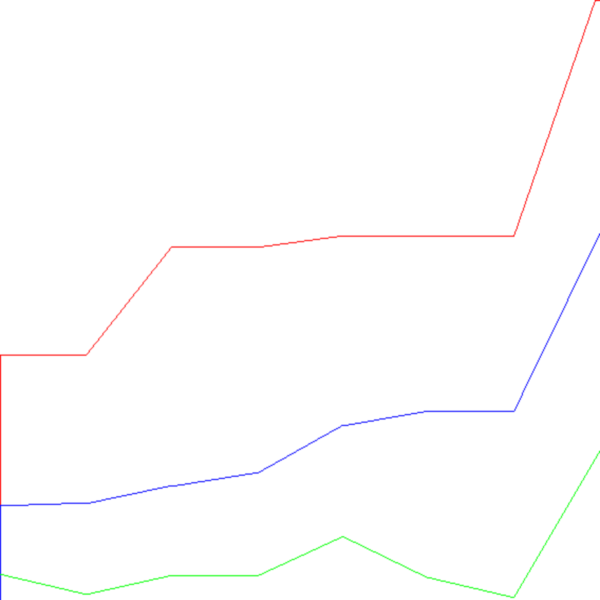
\includegraphics[width=0.3\textwidth]{result_1_1}}
  \subfloat[9.5 After 33 rounds]{\label{fig:result_1_2}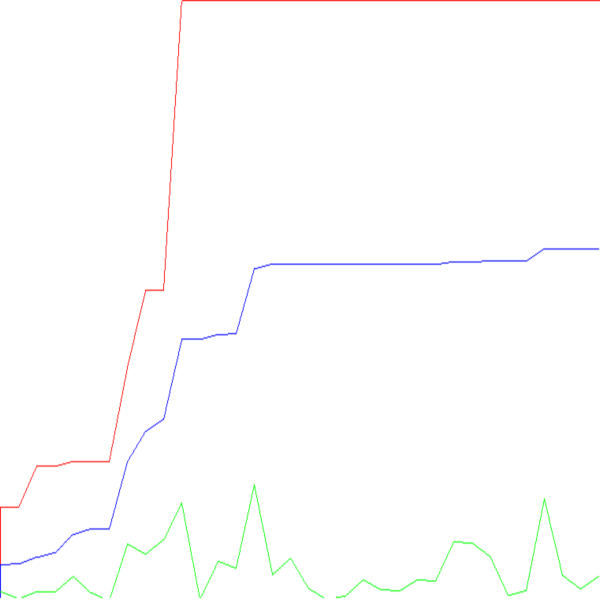
\includegraphics[width=0.3\textwidth]{result_1_2}}
  \subfloat[35 After 65 rounds]{\label{fig:result_1_3}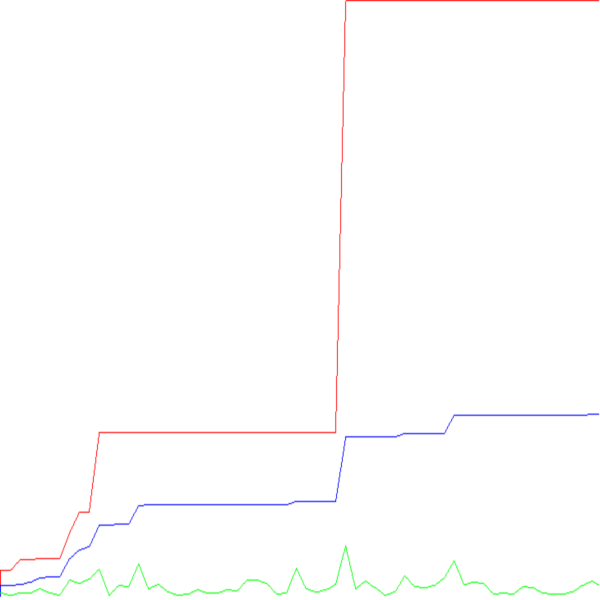
\includegraphics[width=0.3\textwidth]{result_1_3}}
  \caption{Graphical representation of fitness values throughout generations at different times}
  \label{fig:result_1}
\end{figure}

The results clearly show that the highest fitness value remains in the population. It also indicates that the top fitness values remain in the population as the average
does not decrease. However, the average of newly mutated chromosomes is always dissapointingly low. This was thought to be extremely unlikely as one simple mutation should
not have such a major impact that the fitness value drops to zero. In the mean time, the best robots showed promising results! \\

For a while we had no idea what was going on. When we discovered that sometimes the best robot the program wrote to a file wasn't actually the best robot in the program
that we build in a check that reevalutes the complete population every 10 evolution rounds. The result is shown in figure \ref{fig:result_2}.

\begin{figure}[h!]
    \centering
    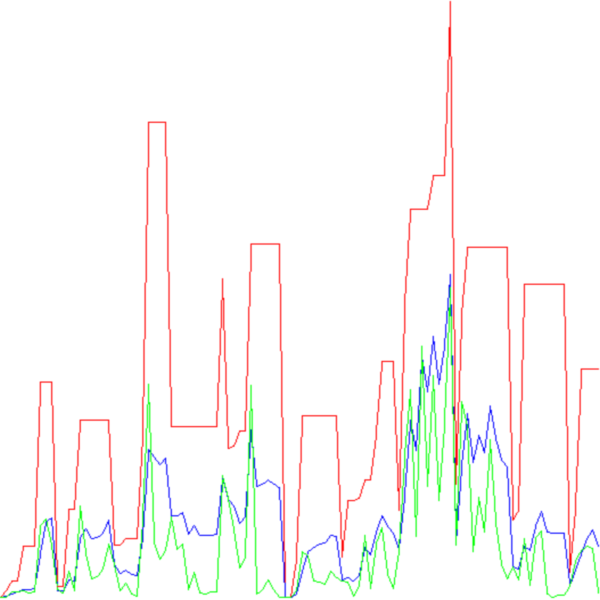
\includegraphics[width=0.5\textwidth]{result_2}
    \caption{The results with a reevaluation every 10 rounds}
    \label{fig:result_2}
\end{figure}

It seemed the fitness value was constant but the chromosomes continued to evolve. After examining our algorithm even further we were still unable to find any bugs. 
When we almost gave up we remembered how Java does not always stores a copy of an object but actually a copy of the reference to the object. This would explain 
everything and with the Java/Eclipse debugger we could validate this. The easy fix was to clone our chromosomes. \\

The first results proved promising but still not what we expected. After more research we learned we had to clone every object, and not just the chromosomes. Our program
stores objects in objects using arrays. We assumed incorrectly cloning the first layer (chromosome) would be sufficient, instead we had to clone up till the deepest 
stored objects in our program. Every layer (see figure \ref{fig:layers}) of our Program had to be cloned in a specific manner. It took us a lot of time to figure out that
 this actually had to be done for each layer. Especially the last layer, the \textit{ExpressionTree} which is recursively stored was tricky. \\

\begin{figure}[h!]
    \centering
    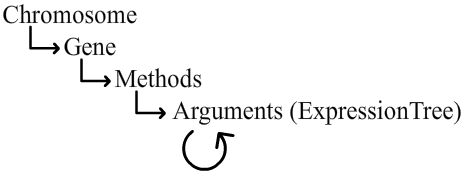
\includegraphics[width=0.5\textwidth]{layers}
    \caption{The depth of our program depends on the depth of an \textit{ExpressionTree}}
    \label{fig:layers}
\end{figure} 

After this ephiphany implementation was easy and we could finally start evolving. As we had expected in the beginning, robots did not devolve and when they did only 
minimally. The results in figure \ref{fig:result_3} clearly shows a rising average fitness value! The ninetieth generation was able to deliver robots that could beat
our default opponent \textit{Spinbot}. We were very happy with this! 

\begin{figure}[h!]
  \centering
  \subfloat[41 After 41 rounds]{\label{fig:result_3_1}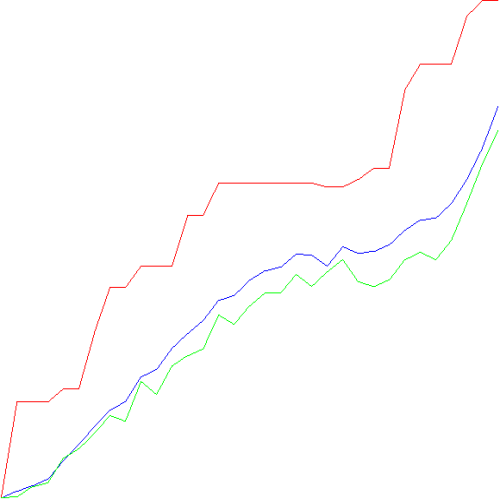
\includegraphics[width=0.4\textwidth]{result_3_1}}
  \subfloat[120 After 102 rounds]{\label{fig:result_3_2}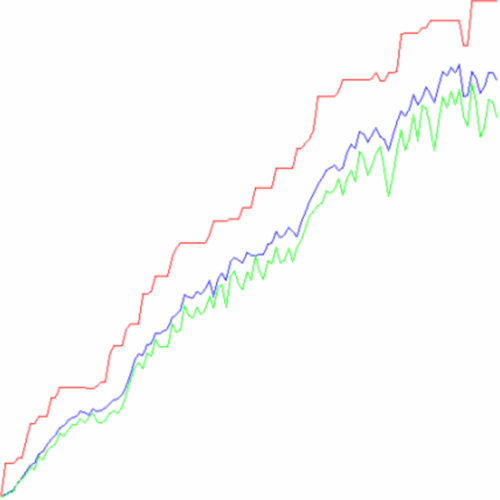
\includegraphics[width=0.4\textwidth]{result_3_2}}
  \caption{Graphical representation of fitness values throughout generations at different times showing correct results.}
  \label{fig:result_3}
\end{figure}

\subsection{Creating our own Framework, a Good Decision?}
% perhaps we should put this in results somehow/somewhere
Creating framework definitely helped us find, identify and solve the problems. Our well structured code now allows us to easily change parameters and even basic 
functioning of 
the program. However, we currently do not know if the unexpected results produced by JGAP were produced by the same kind of programming mistakes. If this is the case some
of the problems might not have been caused by JGAP. \\

While it is easy to change the parameters and basic functioning of the program, changing something more advanced such as the manner on which the program selects the
best genes costs significantly more time. Perhaps even more time in our framework then in it would have had in JGAPs. We had no time left to do this and as a result of
 this the behaviour of a robot is fixed early on. \\

For example, there are multiple efficient methods to gather information. The robot could scan the entire room by turning the radar continuously or the robot could
keep the radar fixed on the target. It is generally accepted that the latter method is more efficient. However, when robots in earlier generations evolve the former 
method it is almost impossible to evolve the different, better method as there are multiple evolution cycles needed to evolve to the different information gathering
 method. In the mean time, while evolving, it has no information gathering method making it extremely unlikely that the robot achieves an high enough fitness value to
survive and evolve further.  \\

There are two things that could fix this. We could select the genes that survive based on their fitness value and a chance or we could implement cross mutation. 

















  
\end{document}
